\paragraph{} Identificados os conflitos e as situações em que estes ocorrem procedeu-se à sua resolução. Para resolver os conflitos \texttt{RAW} foi utilizada a técnica de \textit{forwarding} dos resultados dos andares e execução e de \textit{write back} para o andar de \textit{ID}. No caso dos conflitos de controlo recorreu-se à implementação de uma \textit{Branch Target Buffer}, mas também se considerou a utilização da técnica de \textit{Branch Delay}.

\subsection{Resolução de Conflitos \texttt{RAW}}

\paragraph{} Os conflitos \texttt{RAW} são resolvidos através de caminhos de \textit{forwarding} do andar de \texttt{WB}, da \texttt{ALU} e Memória. Os caminhos tomados são: saída da \texttt{ALU} e da Memória para a saída do andar de \texttt{ID} e saída do andar de \textit{Write Back} para a saída de \texttt{ID}.
Para isso, na saída do andar de \texttt{ID} são colocados \textit{multiplexers} de forma a seleccionar o operando correcto.

Para verificar se existe um conflito deste tipo são verificados os operandos a ser usados, o operando de destino e o sinal de \textit{write enable}, em todos os andares de \textit{pipeline}.

Foram implementadas duas configurações de \textit{forwarding} uma com \textit{forwarding} na saída da Memória de Dados e outra sem. 

Verificou-se que com a introdução de um caminho de \textit{forwarding} da saída da Memória de Dados até ao andar de ID, este fazia parte do caminho crítico. Desta forma optou-se por implementar uma segunda configuração sem este caminho de \textit{forwarding}. Esta solução apresenta algumas vantagens uma vez que permite ter uma frequência máxima de funcionamento mais elevada, embora resulte num maior número de \textit{stalls} mais elevado, introduzido quando se tem instruções de \textit{Load} da memória. De qualquer forma, esta desvantagem pode ser colmatada com o auxílio do compilador através da reordenação de algumas instruções de forma a minimizar o número de \textit{stalls} introduzido devido há não existência de \textit{forwarding} nas instruções de \textit{Load}.

A primeira solução apresenta a vantagem de não necessitar da ajuda do compilador para reduzir o número de \textit{stalls}, o que nem sempre é possível, mas apresenta uma frequência máxima de funcionamento mais baixa.

\paragraph{} A Tabela \ref{tab:forward} \footnote{São usados os testes providenciados pelo professor na página da UC ao longo do relatório.} apresenta os resultados obtidos com e sem o caminho (todos os resultados apresentados em ciclos)\footnote{Assumindo \texttt{BTB} de 2 bits.}:

% inserir tabelas de comparações
\begin{table}[H]
  \caption{Resultados obtidos para a Memória}
  \label{tab:forward}
  \centering  
  \begin{tabular}{| l | c | c | c | c |}
  	\hline
     &
    \multicolumn{1}{c|}{Sem \textit{forwarding}} & 
    \multicolumn{1}{c|}{Com \textit{forwarding}} \\ \hline
    \textbf{Programa} & \textbf{Total} & \textbf{Total} \\ \hline
	Teste 1 & 57   & 57   \\ \hline
    Teste 2 & 2449 & 2359 \\ \hline
    Teste 3 & 1204 & 1099 \\
	\hline
  \end{tabular}
\end{table}

A partir destes resultados pode-se confirmar que o compilador não está a fazer a reordenação esperada gerando \textit{stalls} entre instruções resultando em, alguns casos, numa diferença de 100 ciclos, entre a configuração com caminho e sem caminho. Também de notar que muitos dos \textit{stalls} gerados são devidos a conflitos de controlo que vão ser descritos a seguir.

\subsection{Resolução de Conflitos de Controlo}

\paragraph{} Para resolver os conflitos de controlo foram consideradas 2 técnicas diferentes: \textit{Branch Delay} e a utilização de uma \texttt{BTB} (\textit{Branch Target Buffer}) com um ou mais bits de predição. Todos com predição local.

\subsubsection{\textit{Branch Delay}}
\paragraph{} A técnica de \textit{Branch Delay} adiciona uma instrução depois de uma instrução de controlo que é sempre executada, sendo esta útil ou não. É deixada à responsabilidade do compilador utilizar esta instrução adicional para executar uma instrução útil sempre que possível. Com este método e com 1 \textit{slot}, se o cálculo do endereço de destino for no andar de \texttt{EX/MEM} e não houver \textit{forward} de \textit{flags}, é sempre necessário inserir um \textit{stall} depois da instrução extra. Como o \textmu RISC apresenta uma profundidade de \textit{pipeline} muito pequena este problema podia ser facilmente resolvido com a adição de outro \textit{slot} ou com \textit{forward} das \textit{flags} para o andar de \texttt{ID}, resultando na resolução do salto um andar antes. Mas, a arquitectura fica altamente dependente da competência do compilador de colocar no \textit{slot} uma instrução útil em vez de um \textit{NOP} o que nem sempre é possível.

\subsubsection{\textit{Branch Target Buffer}}

\paragraph{} O \textit{Branch Target Buffer} tal como o nome indica prevê o resultado do salto através do valor dos bits de predição. Cada combinação de bits é um estado que indica se se deve saltar ou não, quantos mais bits se adicionam mais estados se tem. Isto permite antecipar a ocorrência de um salto antes de fazer a sua verificação. Uma vez que se está a fazer uma previsão pode ocorrer que um salto que foi previsto como tomado se venha a verificar que não era suposto ser tomado e neste caso a instrução lida da memória de instruções foi lida incorrectamente e tem que ser anulada.

Além dos bits de predição, por cada instrução é armazenado na \texttt{BTB} o endereço de salto calculado e uma \textit{tag} composta pelos 8 bits mais significativos do endereço da instrução de salto na memória de instruções de forma a poder verificar se a instrução de salto se encontra armazenada na \texttt{BTB}.

\paragraph{} De forma a que este método seja eficaz a \texttt{BTB} deve ser colocada no andar de \textit{fetch} de forma a que o \textit{program counter} possa ser actualizado com o endereço de salto armazenado na \texttt{BTB} caso seja previsto um salto como tomado.

\paragraph{} Este método é especialmente eficaz, na resolução de conflitos, quando existem muitos \textit{loops} no programa, uma vez que a existência de \textit{loops} leva a um menor número de predições de salto falhadas. Deixam de ser tão eficazes também quando se tem algoritmos complexos que executam muitos \textit{branches} condicionais que estão relacionados.

\paragraph{} Em arquitecturas em que o \textit{pipeline} é muito profundo, o endereço de salto é calculado muito tarde devido ao número elevado de andares entre o andar de \textit{fetch} e o andar onde o salto é resolvido, este método é mais eficaz uma vez que permite reduzir muitos \textit{stalls} introduzidos entre o andar de \textit{fetch} e o andar onde se resolve o salto.

\paragraph{} Foram implementados dois esquemas de predição de salto um com apenas 1 bit de predição e outro com 2 bits de predição, com o objectivo de poder comparar a performance das duas soluções. A máquina de estados do \textit{branch prediction buffer} com 1 bit e 2 bits encontram-se demonstradas na Figura \ref{fig:bpb1} e na Figura \ref{fig:bpb2}\footnote{Imagens retiradas dos slides utilizados nas aulas teóricas}, respectivamente.

\begin{figure}[H]
    \centering
    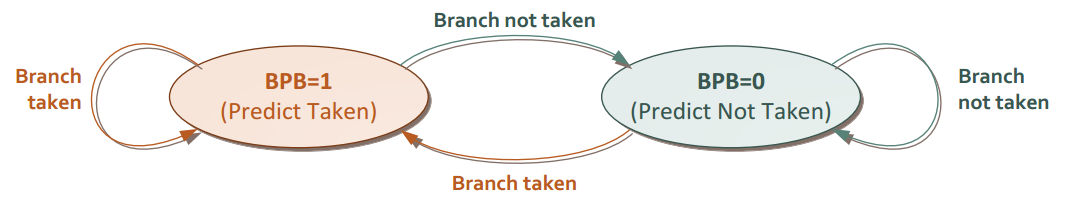
\includegraphics[width=0.8\textwidth]{./btb1bit.png}~\\[1cm]
    \caption{Máquina de Estados do BPB de 1 bit}
    \label{fig:bpb1}
\end{figure}

\begin{figure}[H]
    \centering
    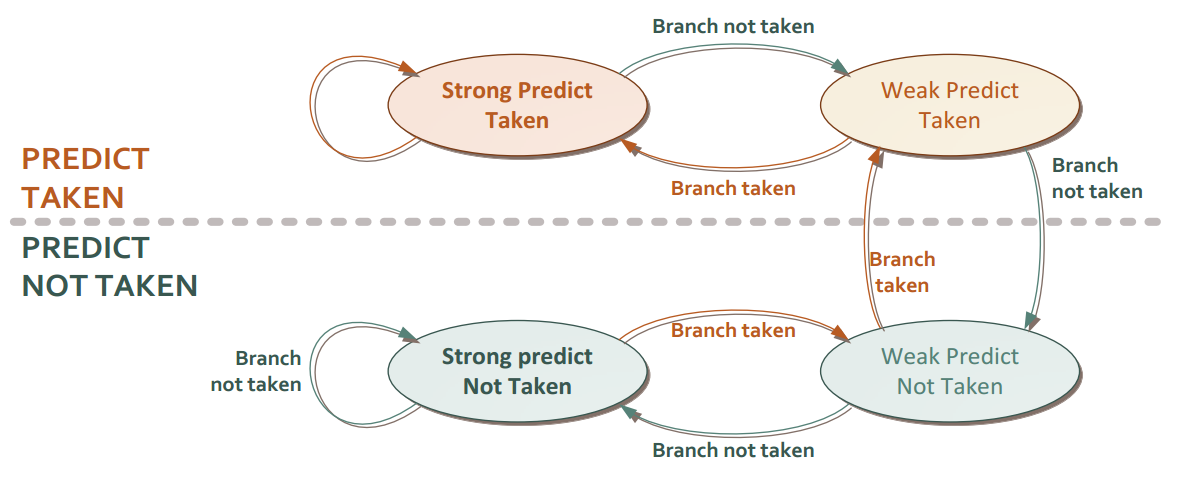
\includegraphics[width=0.8\textwidth]{./btb2bit.png}~\\[1cm]
    \caption{Máquina de Estados do BPB de 2 bit}
    \label{fig:bpb2}
\end{figure}

Os resultados para as duas implementações estão presentes na Tabela \ref{tab:BTB}\footnote{Assumindo \textit{forward} de memória.}.

\begin{table}[H]
  \caption{Resultados obtidos para a \texttt{BTB} de 1 e 2 bits}
  \label{tab:BTB}
  \centering  
  \begin{tabular}{| l | c | c | c | c |}
  	\hline
     & 
    \multicolumn{2}{c|}{\texttt{BTB} de 1 bits} &
    \multicolumn{2}{c|}{\texttt{BTB} de 2 bits} \\ \hline
    \textbf{Programa} & \textbf{Total} & \textbf{Falhas de Predição} & \textbf{Total} & \textbf{Falhas de Predição} \\ \hline
	Teste 1 & 57   & 0   & 57   & 0\\ \hline
    Teste 2 & 2359 & 108 & 2349 & 97\\ \hline
    Teste 3 & 1099 & 122 & 1098 & 121\\
	\hline
  \end{tabular}
\end{table}


